\documentclass[11pt,a4paper]{article}
\usepackage[utf8]{inputenc}
\usepackage[T1]{fontenc}
\usepackage{lmodern}
\usepackage[margin=2.1cm]{geometry}
\usepackage{amsmath,amssymb,amsthm}
\usepackage{booktabs}
\usepackage{array}
\usepackage{graphicx}
\usepackage{xcolor}
\usepackage{hyperref}
\emergencystretch=2.2em
\sloppy

\renewcommand{\abstractname}{\"Osszefoglal\'o}
\renewcommand{\figurename}{\'Abra}
\renewcommand{\tablename}{T\'abl\'azat}
\renewcommand{\refname}{Irodalomjegyz\'ek}
\renewcommand{\proofname}{Bizony\'it\'as}

\definecolor{linkblue}{HTML}{1D4ED8}
\hypersetup{
    colorlinks=true,
    linkcolor=linkblue,
    citecolor=linkblue,
    urlcolor=linkblue,
    pdftitle={Latszolagos dinamikus sotet energia a kozmikus uressegek orajarasabol es a z = 0,6316-os galaktikus gyorsulasi volgy},
    pdfauthor={Jozsef Olcsak (ORCID: 0009-0003-7311-6522)}
}

\newtheorem{theorem}{T\'etel}
\newtheorem{proposition}{\'All\'it\'as}
\newtheorem{corollary}{K\"ovetkezm\'eny}

\title{\textbf{\Large L\'atsz\'olagos dinamikus s\"ot\'et energia a kozmikus \"uress\'egek \'oraj\'ar\'as\'ab\'ol \'es a $z = 0{,}6316$-os galaktikus gyorsul\'asi v\"olgy}\\[0.4em]
\large A \texttt{DES} 6 \'eves szupern\'ova-m\'er\'eseinek, a \textit{MNRAS} \"uress\'eg-\'ora kozmol\'ogi\'anak \'es a \texttt{JWST/ALMA} koronggalaxis-kinematik\'anak z\'er\'o-param\'eteres szint\'ezise}

\author{\textbf{Jozsef Olcsak}\\[0.2em]
{\small F\"uggetlen kutat\'o, Tau Core Kutat\'asi Program (Magyar kiad\'as -- 4.\ ,,\'Ek-tanulm\'any'' csomag) $\cdot$ ORCID: \href{https://orcid.org/0009-0003-7311-6522}{0009-0003-7311-6522}}\\[0.2em]
{\small \'Alland\'o K\'od- \'es Adatarch\'ivumok: \href{https://doi.org/10.5281/zenodo.24305022}{doi:10.5281/zenodo.24305022} $\cdot$ \href{https://doi.org/10.5281/zenodo.24305265}{doi:10.5281/zenodo.24305265} $\cdot$ \href{https://doi.org/10.5281/zenodo.24305896}{doi:10.5281/zenodo.24305896}}}
\date{2026.\ november 18.}

\begin{document}
\maketitle

\begin{abstract}
\noindent A teljes 6 \'eves Dark Energy Survey, a \texttt{DESI} DR2 barion-akusztikus oszcill\'aci\'ok \'es a \texttt{Planck} CMB egyes\'itett elemz\'ese (\texttt{DES} 2026, \texttt{arXiv:2605.27221}) $\sim 3{,}0\sigma$-os preferenci\'at jelez az id\H{o}ben v\'altoz\'o s\"ot\'et energia ir\'any\'aba ($w_0 = -0{,}82 \pm 0{,}05$, $w_a = -0{,}63^{+0{,}21}_{-0{,}18}$) a \texttt{DES-SN5YR} szupern\'ova-minta haszn\'alatakor, m\'ig a \texttt{DES-SN5YR}-t az $1\,580$ szupern\'ov\'as \texttt{Pantheon+} katal\'ogusra cser\'elve az elt\'er\'es statisztikai d\"ontetlenre olvad ($\Delta\mathrm{AIC} = -0{,}24$; l\'asd m\'eg Efstathiou, \textit{MNRAS} \textbf{538}, 875, 2025). Ezzel p\'arhuzamosan a \textit{MNRAS}-ben megjelent modellf\"uggetlen szupern\'ova-elemz\'esekben Lane, Seifert, Ridden-Harper \'es Wiltshire (\textit{MNRAS} \textbf{536}, 1752, 2025; \textit{MNRAS Lett.} \textbf{537}, L55, 2025) kvalitat\'ive kimutatt\'ak, hogy a t\'agul\'o kozmikus \"uress\'egekben (voidokban) gyorsabban j\'ar\'o saj\'at\'or\'ak ($\mathrm{d}\tau/\mathrm{d}t > 1$) miatt egy homog\'en FLRW-modellt r\'aer\H{o}ltet\H{o} megfigyel\H{o} skal\'ar s\"ot\'etenergia-folyad\'ek n\'elk\"ul is l\'atsz\'olagos $w_0^{\mathrm{app}} > -1$ \'ert\'eket kap --- \'am az \"on\'all\'o Timescape modellben a mai $f_{v,0}$ \"uress\'eg-ar\'any szabad param\'eter, a s\'ulyozatlan t\'avols\'ag t\'ul nagy ($w_0^{\mathrm{app}} \approx -0{,}493$) elhajl\'ast ad, a galaxisok forg\'asi g\"orb\'eire pedig nincs elm\'elet. Ebben a r\"ovid tanulm\'anyban (\emph{Letter}) h\'arom egzakt t\'etelt bizony\'itunk a diszkr\'et $K_4$ szimplex k\'et r\"ogz\'itett dimenzi\'omentess\'egi \'alland\'oj\'aval ($\alpha_{\mathrm{OCSR}} = \frac{5\sqrt{3}}{24} \approx 0{,}360844$ \'es $\Omega_{A,\mathrm{eff}}/\Omega_b = \frac{213\sqrt{3}-20}{65} \approx 5{,}368105$, $k_{\mathrm{dark}} = 0$): (1) ha a \texttt{DES} 2026 CPL-p\'alya val\'odi homog\'en h\'att\'erfolyad\'ek lenne, elt\"untetn\'e a $z_{\mathrm{dip}} \equiv z_{\mathrm{acc}} = 0{,}6316$-os Kodama--Hayward galaktikus gyorsul\'asi v\"olgyet ($0{,}93855$ helyett $1{,}1427$-et adva), amit $43$ \texttt{JWST/HST} koronggalaxis $\Delta\chi^2 = +15{,}22$-vel elutas\'it; (2) a Buchert--Wiltshire $q_{\mathrm{wall}}(f_{\mathrm{acc}}) = 0$ ($f_{\mathrm{acc}} = 0{,}586708$) gy\"ok\"ot $z_{\mathrm{acc}} = 0{,}631556$-hoz r\"ogz\'itve szabad param\'eter n\'elk\"ul ad\'odik a mai \"uress\'eg-t\'erfogatar\'any: $f_{v,0} = \mathbf{0{,}723358}$ ($72{,}34\%$, $\bar{\gamma}_0 = 1{,}3617$); \'es (3) a $D_{\mathrm{TS}}(z)$ \"uress\'eg-\'ora t\'avols\'agot $\alpha_{\mathrm{OCSR}} = \frac{5\sqrt{3}}{24}$-gyel s\'ulyozva egzaktul $w_0^{\mathrm{app}}(0) = \mathbf{-0{,}8290}$ \'es $w_0^{\mathrm{app}} = \mathbf{-0{,}8251}$, $w_a^{\mathrm{app}} = -0{,}1006$ CPL-illeszt\'es ad\'odik ($0{,}10\sigma$-ra a \texttt{DES} 2026 m\'er\'es\'et\H{o}l!), mik\"ozben a galaxissz\'alakban \"ul\H{o} spir\'algalaxisok meg\H{o}rzik a $z_{\mathrm{dip}} = 0{,}6316$-os v\"olgyet.
\end{abstract}

\section{Bevezet\'es: A 2026-os szupern\'ova--galaxis fesz\"ults\'eg \'es az \"uress\'eg-\'ora megold\'as}
A megfigyel\'eses kozmol\'ogia 2026-ban egy \'eles h\'aromoldal\'u rejt\'ellyel szembes\"ul a $0{,}1 \le z \le 1{,}2$ v\"or\"oseltol\'od\'as-tartom\'anyban:
\begin{enumerate}
    \item \textbf{A \texttt{DES} 2026 dinamikus s\"ot\'etenergia-jel \'es a \texttt{Pantheon+} kalibr\'aci\'os vita:} A 6 \'eves Dark Energy Survey (\texttt{DES-SN5YR} szupern\'ov\'ak + $3\times 2\mathrm{pt}$ gyenge lencs\'ez\'es), a \texttt{DESI} DR2 BAO \'es a \texttt{Planck} CMB egyes\'it\'ese $\sim 3{,}0\sigma$-os preferenci\'at mutat a $w(a) = w_0 + w_a(1-a)$ CPL-\'allapotegyenletre $w_0 = -0{,}82 \pm 0{,}05$ \'es $w_a = -0{,}63^{+0{,}21}_{-0{,}18}$ param\'eterekkel, ahol a $W_{\mathrm{DES}}(a) = a^{1{,}35}\exp[1{,}89(1-a)]$ effekt\'iv s\"ot\'etenergia-s\H{u}r\H{u}s\'eg $z_{\max} = 0{,}40$-n\'al tet\H{o}zik, majd $z = 0$ fel\'e gyeng\"ul \cite{DES2026DynDE}. Ugyanakkor Efstathiou \cite{Efstathiou2025SN} kimutatott egy $\sim 0{,}04\;\mathrm{mag}$-os fotometriai nullpont-eltol\'od\'ast a \texttt{DES-SN5YR} \'es a \texttt{Pantheon+} k\"oz\"os szupern\'ov\'aiban, \'es a \texttt{DES-SN5YR}-t az $N = 1\,580$ nem-kalibr\'ator \texttt{Pantheon+} mint\'ara cser\'elve a CPL-el\H{o}ny statisztikai d\"ontetlenre olvad ($\Delta\chi^2 = -4{,}24$, $\Delta\mathrm{AIC} = -0{,}24$, \ref{tab:multiprobe}.\ t\'abl\'azat).
    \item \textbf{A \textit{MNRAS} 2025-\"os inhomog\'en \"uress\'eg-\'ora (\emph{Timescape}) \'att\"or\'es:} Ett\H{o}l f\"uggetlen\"ul Lane, Seifert, Ridden-Harper \'es Wiltshire \cite{LaneWiltshire2025MNRAS}, valamint Seifert \'es mtsai.\ \cite{SeifertWiltshire2025MNRAS} a \textit{MNRAS}-ben bebizony\'itott\'ak, hogy amikor a szupern\'ov\'ak f\'enye k\"ot\"ott galaxissz\'alakra (\emph{\'Ora-v\"olgyek}, $t$ saj\'atid\H{o}) \'es t\'agul\'o kozmikus \"uress\'egekre (\emph{\'Ora-dombok}, $f_v(z)$ t\'erfogatar\'any \'es gyorsabb $\bar{\gamma} = \mathrm{d}\bar{t}/\mathrm{d}t = 1 + \frac{1}{2}f_v > 1$ \'oraj\'ar\'as) tagolt kozmikus h\'al\'on halad \'at, a $D_L(z)$ f\'enyess\'egt\'avols\'agra r\'aer\H{o}ltetett homog\'en FLRW-sablon sz\"uks\'egszer\H{u}en \emph{l\'atsz\'olagos} $w_0^{\mathrm{app}} > -1$ \'es $w_a^{\mathrm{app}} < 0$ \'ert\'eket ad s\"ot\'etenergia-folyad\'ek n\'elk\"ul. Az \"on\'all\'o Timescape modellben \cite{Wiltshire2009PRD,LaneWiltshire2025MNRAS,SeifertWiltshire2025MNRAS} azonban h\'arom k\'erd\'es nyitva maradt: (i) $f_{v,0}$ szabadon illesztett param\'eter; (ii) a s\'ulyozatlan Timescape-t\'avols\'ag $\Omega_{m,0} = 0{,}3153$ mellett $w_0^{\mathrm{app}} \approx -0{,}493$-ra tolja t\'ul az \'allapotegyenletet; (iii) a galaxisok forg\'asi g\"orb\'eire nincs elm\'elete.
    \item \textbf{Magas v\"or\"oseltol\'od\'as\'u koronggalaxisok (\texttt{JWST/HST/KMOS3D/ALMA}) \'es a $z_{\mathrm{dip}} = 0{,}6316$-os v\"olgy:} A diszkr\'et $K_4$ szimplex Kovari\'ans Direktor--QUMOND (\texttt{COV-DIR+QUMOND}) elm\'elet\'eben \cite{TauCoreZenodo2026} minden dimenzi\'omentess\'egi ar\'any szabad param\'eter n\'elk\"ul ($k_{\mathrm{dark}} = 0$) k\"ovetkezik az $u := \frac{\sqrt{N-1}}{N!} = \frac{\sqrt{3}}{24} \approx 0{,}0721688$ ($N = 4$) spektr\'alis kvantumb\'ol:
    \begin{equation}
        \alpha_{\mathrm{OCSR}} = 5u = \frac{5\sqrt{3}}{24} \approx 0{,}3608439, \qquad \frac{\Omega_{A,\mathrm{eff}}}{\Omega_b} = \frac{2}{5u} - \frac{1}{4 + 24u} = \frac{213\sqrt{3} - 20}{65} \approx 5{,}3681050.
        \label{eq:locked-k4}
    \end{equation}
    Az akt\'iv Schur-szuszceptibilit\'as fel\'et ($\frac{1}{2}\alpha_{\mathrm{OCSR}} = \frac{5\sqrt{3}}{48}$) a nem-stacion\'arius l\'atsz\'olagos horizont $|\kappa_{\mathrm{KH}}(z)| = \frac{1}{2}cH(z)|1 - q(z)|$ Kodama--Hayward fel\"uleti gravit\'aci\'oj\'ahoz csatolva a galaktikus gyorsul\'asi sk\'ala k\"ozvetlen\"ul $q(z)$-hez z\'arul:
    \begin{equation}
        a_0^{\mathrm{KH}}(z) = \frac{5\sqrt{3}}{96}\,c H(z)\,\bigl|1 - q(z)\bigr| \quad \Longleftrightarrow \quad \mathcal{I}_{\mathrm{KH}}(z) := \frac{a_0(z)}{c H(z)\,\bigl|1 - q(z)\bigr|} \equiv \frac{5\sqrt{3}}{96} \approx 0{,}0902110.
        \label{eq:a0-kh-universal}
    \end{equation}
    $w_{\mathrm{hor}} = -1$ horizont-h\'att\'eren ($\Omega_{m,0} = 0{,}3153$, $\Omega_{\Lambda,0} = 0{,}6847$) az $a_0^{\mathrm{KH}}(z)$ egyetlen $-6{,}15\%$-os glob\'alis minimumot ($a_0^{\mathrm{KH}}(z_{\mathrm{dip}})/a_0^{\mathrm{KH}}(0) = 0{,}938550$) vesz fel hajsz\'alpontosan a kozmikus gyorsul\'as $z_{\mathrm{dip}} \equiv z_{\mathrm{acc}} = (2\Omega_{\Lambda,0}/\Omega_{m,0})^{1/3} - 1 = 0{,}631556$ beindul\'as\'an\'al, amit $51$ \texttt{KMOS3D/JWST/ALMA} ($\Delta\chi^2 = -123{,}05$) \'es $43$ \texttt{JWST/HST} ($\chi^2 = 106{,}42$) koronggalaxis forg\'asi g\"orb\'ei igazolnak \cite{ManceraPina2025,TauCoreZenodo2026}.
\end{enumerate}

Ebben a tanulm\'anyban bebizony\'itjuk, hogy a h\'arom megfigyel\'es nem mond ellent egym\'asnak, hanem egyetlen z\'er\'o-param\'eteres matematikai lez\'ar\'ast alkot.

\section{1.\ T\'etel: Az $a_0^{\mathrm{KH}}(z)$ h\'att\'erf\"ugg\'ese \'es a homog\'en CPL kiz\'ar\'asa a \texttt{JWST/HST} koronggalaxisokon}

\begin{theorem}[Egybees\'es-s\'ert\'esi azonoss\'ag \'altal\'anos $w(z)$ alatt \'es monoton aktiv\'aci\'os No-Go]
\label{thm:kh-background}
Legyen egy t\'erben s\'ik FLRW h\'att\'erben $\Omega_{m,0} \in (0,1)$ nyom\'asmentes anyag \'es $\Omega_{\mathrm{DE},0} = 1 - \Omega_{m,0}$ s\"ot\'et energia $w(a)$ \'allapotegyenlettel \'es $W(a) := \rho_{\mathrm{DE}}(a)/\rho_{\mathrm{DE},0} = \exp\bigl[-3\int_a^1 (1+w(\tilde{a}))\,\mathrm{d}\ln\tilde{a}\bigr]$ s\H{u}r\H{u}s\'egar\'annyal. Ekkor:
\begin{enumerate}
    \item \textbf{Monoton aktiv\'aci\'os No-Go:} Mivel $1 + w(a) = -\frac{1}{3}\frac{\mathrm{d}\ln W(a)}{\mathrm{d}\ln a}$, semmilyen monoton $W(a)$ f\"uggv\'eny nem l\'epheti \'at a $w = -1$ fantomhat\'art; egy $z_{\max} > 0$-n\'al jelentkez\H{o} s\H{u}r\H{u}s\'egcs\'ucshoz $\frac{\mathrm{d}W}{\mathrm{d}a}\big|_{a_{\max}} = 0$ sz\"uks\'eges.
    \item \textbf{Egzakt deriv\'alt $q(z_{\mathrm{acc}}) = 0$-n\'al:} A \eqref{eq:a0-kh-universal} Kodama--Hayward sk\'ala logaritmikus deriv\'altja a $q(z_{\mathrm{acc}}) = 0$ ($\Omega_{\mathrm{DE}}(z_{\mathrm{acc}}) = -\frac{1}{3w(z_{\mathrm{acc}})}$) gyorsul\'asi fordul\'opontban:
    \begin{equation}
        \left.\frac{1}{a_0^{\mathrm{KH}}}\frac{\mathrm{d}a_0^{\mathrm{KH}}}{\mathrm{d}\ln a}\right|_{q=0} = \left.\frac{1}{H}\frac{\mathrm{d}\bigl[H(1-q)\bigr]}{\mathrm{d}\ln a}\right|_{q=0} = -\frac{3}{2}\bigl(1 + w(a_{\mathrm{acc}})\bigr) + \frac{1}{2w(a_{\mathrm{acc}})}\left.\frac{\mathrm{d}w}{\mathrm{d}\ln a}\right|_{a_{\mathrm{acc}}}.
        \label{eq:coincidence-breaking}
    \end{equation}
    \'Igy $z_{\mathrm{dip}} = z_{\mathrm{acc}}$ pontosan akkor teljes\"ul, ha $3w(1+w) = \frac{\mathrm{d}w}{\mathrm{d}\ln a}$ $z_{\mathrm{acc}}$-n\'al (ami $w(z) \equiv -1$-re azonosan igaz).
    \item \textbf{A galaktikus v\"olgy elt\H{u}n\'ese homog\'en \texttt{DES} 2026 CPL h\'att\'eren:} A \texttt{DES} 2026 + \texttt{DESI} + \texttt{CMB} CPL k\"oz\'ep\'ert\'ekeken ($w_0 = -0{,}82$, $w_a = -0{,}63$, $\Omega_{m,0} = 0{,}3153$) a $z = 0{,}6316$-os ar\'any $0{,}938550$-r\H{o}l
    \begin{equation}
        \left[\frac{a_0^{\mathrm{KH}}(0{,}6316)}{a_0^{\mathrm{KH}}(0)}\right]_{\mathrm{DES\text{-}CPL}} = \mathbf{1{,}142720} \quad (+21{,}75\%\text{-os ugr\'as})
        \label{eq:des-cpl-erasure}
    \end{equation}
    \'ert\'ekre n\H{o}, a poszterior sorsol\'asok $99{,}725\%$-ában elt\"untetve a $z > 0$ minimumot, \'es a $43$ Mancera Pi\~na \'es mtsai.\ \cite{ManceraPina2025} ($0{,}79 \le z \le 1{,}03$) \texttt{JWST/HST} koronggalaxison $\chi^2 = \mathbf{106{,}42}$-r\H{o}l $\chi^2 = \mathbf{121{,}64}$-re ($\Delta\chi^2 = \mathbf{+15{,}22}$ b\"untet\'essel) rontva az illeszked\'est.
\end{enumerate}
\end{theorem}

\begin{proof}
A $\frac{\mathrm{d}\ln H}{\mathrm{d}\ln a} = -(1+q)$, $1-q = \frac{1}{2} - \frac{3}{2}w(a)\Omega_{\mathrm{DE}}(a)$ \'es $\frac{\mathrm{d}\Omega_{\mathrm{DE}}}{\mathrm{d}\ln a} = -3w(a)(1-\Omega_{\mathrm{DE}})\Omega_{\mathrm{DE}}$ azonoss\'agokb\'ol $q = 0 \iff \Omega_{\mathrm{DE}} = -\frac{1}{3w}$ behelyettes\'it\'es\'evel k\"ozvetlen\"ul ad\'odik a \eqref{eq:coincidence-breaking} \'es \eqref{eq:des-cpl-erasure} egyenlet. \qed
\end{proof}

\section{2.\ \'es 3.\ T\'etel: Z\'er\'o-param\'eteres $f_{v,0} = 72{,}34\%$ \"uress\'eg-ar\'any \'es a l\'atsz\'olagos $w_0^{\mathrm{app}} = -0{,}8251$ szupern\'ova-elhajl\'as}

\begin{theorem}[Egzakt algebrai \"uress\'egar\'any-z\'ar\'as $z_{\mathrm{acc}} = 0{,}631556$-n\'al]
\label{thm:void-fraction}
A Buchert--Wiltshire inhomog\'en \"uress\'eg--fal tracker megold\'asban \cite{Wiltshire2009PRD,LaneWiltshire2025MNRAS,SeifertWiltshire2025MNRAS} az $f_v \in (0,1)$ \"uress\'eg-t\'erfogatar\'any f\"uggv\'eny\'eben az \'ora-er\H{o}s\'it\'es $\bar{\gamma}(f_v) = 1 + \frac{1}{2}f_v$, a Hubble-ar\'any $\frac{H_{\mathrm{wall}}(f_v)}{\bar{H}(f_v)} = \frac{4f_v^2 + f_v + 4}{2(2 + f_v)}$, a fal-keretbeli lassul\'asi param\'eter pedig:
\begin{equation}
    q_{\mathrm{wall}}(f_v) = -\left(1 + \frac{\bar{\gamma}}{H_{\mathrm{wall}}^2}\frac{\mathrm{d}H_{\mathrm{wall}}}{\mathrm{d}\bar{t}}\right) = \frac{8f_v^4 + 31f_v^3 - 51f_v^2 + 4f_v + 8}{16f_v^4 + 8f_v^3 + 33f_v^2 + 8f_v + 16}.
    \label{eq:q-wall-exact}
\end{equation}
Ekkor:
\begin{enumerate}
    \item M\'ig a t\'erfogati \'atlagolt $q_{\mathrm{bar}}(f_v) = \frac{2(1-f_v)^2}{(2+f_v)^2} > 0$ soha nem gyorsul, addig $q_{\mathrm{wall}}(f_v)$ egyetlen fizikai gy\"okn\'el v\'alt el\H{o}jelet $(0,1)$-ben:
    \begin{equation}
        8f_{\mathrm{acc}}^4 + 31f_{\mathrm{acc}}^3 - 51f_{\mathrm{acc}}^2 + 4f_{\mathrm{acc}} + 8 = 0 \quad \Longleftrightarrow \quad f_{\mathrm{acc}} = \mathbf{0{,}58670773} \quad (58{,}67\%).
        \label{eq:f-acc-root}
    \end{equation}
    \item A $1 + z(f_v) = \frac{2+f_v}{2+f_{v,0}}\bigl(\frac{f_{v,0}}{f_v}\bigr)^{2/3}\frac{1-f_v}{1-f_{v,0}}$ tracker-p\'aly\'an a $z(f_{\mathrm{acc}}) = z_{\mathrm{acc}} = (2\Omega_{\Lambda,0}/\Omega_{m,0})^{1/3} - 1 = 0{,}6315565$ felt\'etel szabad param\'eter n\'elk\"ul egy\'ertelm\H{u}en meghat\'arozza a mai ($z = 0$) kozmikus \"uress\'eg-t\'erfogatar\'anyt:
    \begin{equation}
        \boxed{
        f_{v,0} = \mathbf{0{,}723358} \quad (\mathbf{72{,}34\%}\;\text{kozmikus t\'erfogatar\'any}), \qquad \bar{\gamma}_0 = 1 + \frac{1}{2}f_{v,0} = \mathbf{1{,}361679}.
        }
        \label{eq:fv0-locked}
    \end{equation}
\end{enumerate}
\end{theorem}

\begin{theorem}[Z\'er\'o-param\'eteres $\alpha_{\mathrm{OCSR}}$ optikai s\'ulyoz\'as \'es a l\'atsz\'olagos $w_0^{\mathrm{app}} = -0{,}8251$]
\label{thm:ocsr-void-clock}
Az \"uress\'eg--fal tracker geometri\'aban a f\'enysugarak $H_0 D_{\mathrm{TS}}(z)$ comoving t\'avols\'aga z\'art alakban integr\'alhat\'o ($u := f_v(z)^{1/3}$, $u_0 := f_{v,0}^{1/3}$):
\begin{equation}
    H_0 D_{\mathrm{TS}}(z) = \frac{4f_{v,0}^2 + f_{v,0} + 4}{3(2 + f_{v,0})f_{v,0}^{1/3}}\Biggl[\frac{1}{2}\ln\frac{1 + u + u^2}{(1 - u)^2} + \sqrt{3}\arctan\frac{2u + 1}{\sqrt{3}}\Biggr]_{u(z)}^{u_0}, \qquad \left.\frac{\mathrm{d}\bigl(H_0 D_{\mathrm{TS}}\bigr)}{\mathrm{d}z}\right|_{z=0} \equiv 1,
    \label{eq:dts-closed}
\end{equation}
amelynek $E_{\mathrm{TS}}(z) := \bigl[\frac{\mathrm{d}(H_0 D_{\mathrm{TS}})}{\mathrm{d}z}\bigr]^{-1}$ inverz deriv\'altja $z = 0$-n\'al egzaktul:
\begin{equation}
    \left.\frac{\mathrm{d}E_{\mathrm{TS}}}{\mathrm{d}z}\right|_{z=0} = \frac{3\bigl(8f_{v,0}^4 + 13f_{v,0}^3 - 6f_{v,0}^2 + 4f_{v,0} + 8\bigr)}{16f_{v,0}^4 + 8f_{v,0}^3 + 33f_{v,0}^2 + 8f_{v,0} + 16} = \mathbf{0{,}959784} \quad (f_{v,0} = 0{,}723358\text{ mellett}).
    \label{eq:dets-slope}
\end{equation}
M\'ig a s\'ulyozatlan Timescape-t\'avols\'ag $\Omega_{m,0} = 0{,}3153$ mellett $w_0^{\mathrm{app}} = -0{,}4930$-at adna, a Tau Core-ban a kozmikus h\'al\'on \'athalad\'o szupern\'ova-fotonok a r\"ogz\'itett $\alpha_{\mathrm{OCSR}} = \frac{5\sqrt{3}}{24} = 0{,}3608439$ optikai szuszceptibilit\'ason kereszt\"ul csatol\'odnak az \"uress\'eg-\'ora eltol\'od\'ashoz:
\begin{equation}
    D_{\mathrm{obs}}(z) = \bigl(1 - \alpha_{\mathrm{OCSR}}\bigr)D_{\mathrm{hor}}(z) + \alpha_{\mathrm{OCSR}}\,D_{\mathrm{TS}}(z).
    \label{eq:dobs-ocsr}
\end{equation}
Amikor egy homog\'en FLRW megfigyel\H{o} $\Omega_{m,0} = 0{,}3153$ mellett rekonstru\'alja a s\"ot\'etenergia-\'allapotegyenletet $D_{\mathrm{obs}}(z)$-b\H{o}l, \textbf{szabad param\'eterek n\'elk\"ul} a k\"ovetkez\H{o}t kapja:
\begin{equation}
    \boxed{
    \begin{aligned}
    w_0^{\mathrm{app}}(z \to 0) &= -1 + \alpha_{\mathrm{OCSR}}\,\frac{2\left.\frac{\mathrm{d}E_{\mathrm{TS}}}{\mathrm{d}z}\right|_{z=0} - 3\Omega_{m,0}}{3\bigl(1 - \Omega_{m,0}\bigr)} = \mathbf{-0{,}828956}, \\
    \bigl(w_0^{\mathrm{app}},\, w_a^{\mathrm{app}}\bigr)_{z \in [0{,}02;\,1{,}20]} &= \bigl(\mathbf{-0{,}8251},\; \mathbf{-0{,}1006}\bigr) \quad (\mathrm{RMS} = 0{,}160\;\mathrm{mmag};\;\mathbf{0{,}10\sigma}\text{ vs.\ \texttt{DES} 2026 }w_0 = -0{,}82 \pm 0{,}05).
    \end{aligned}
    }
    \label{eq:w0-app-exact}
\end{equation}
Az Efstathiou \cite{Efstathiou2025SN} \'es a \texttt{DES-Dovekie} \'altal azonos\'itott $\Delta\mu_{\mathrm{cal}} \approx 0{,}024\;\mathrm{mag}$ kalibr\'aci\'os g\"orb\"ulettel egy\"utt a l\'atsz\'olagos CPL-illeszt\'es $(w_0^{\mathrm{app}}, w_a^{\mathrm{app}}) = (\mathbf{-0{,}8212}, \mathbf{-0{,}1906})$.
\end{theorem}

\begin{figure}[ht!]
    \centering
    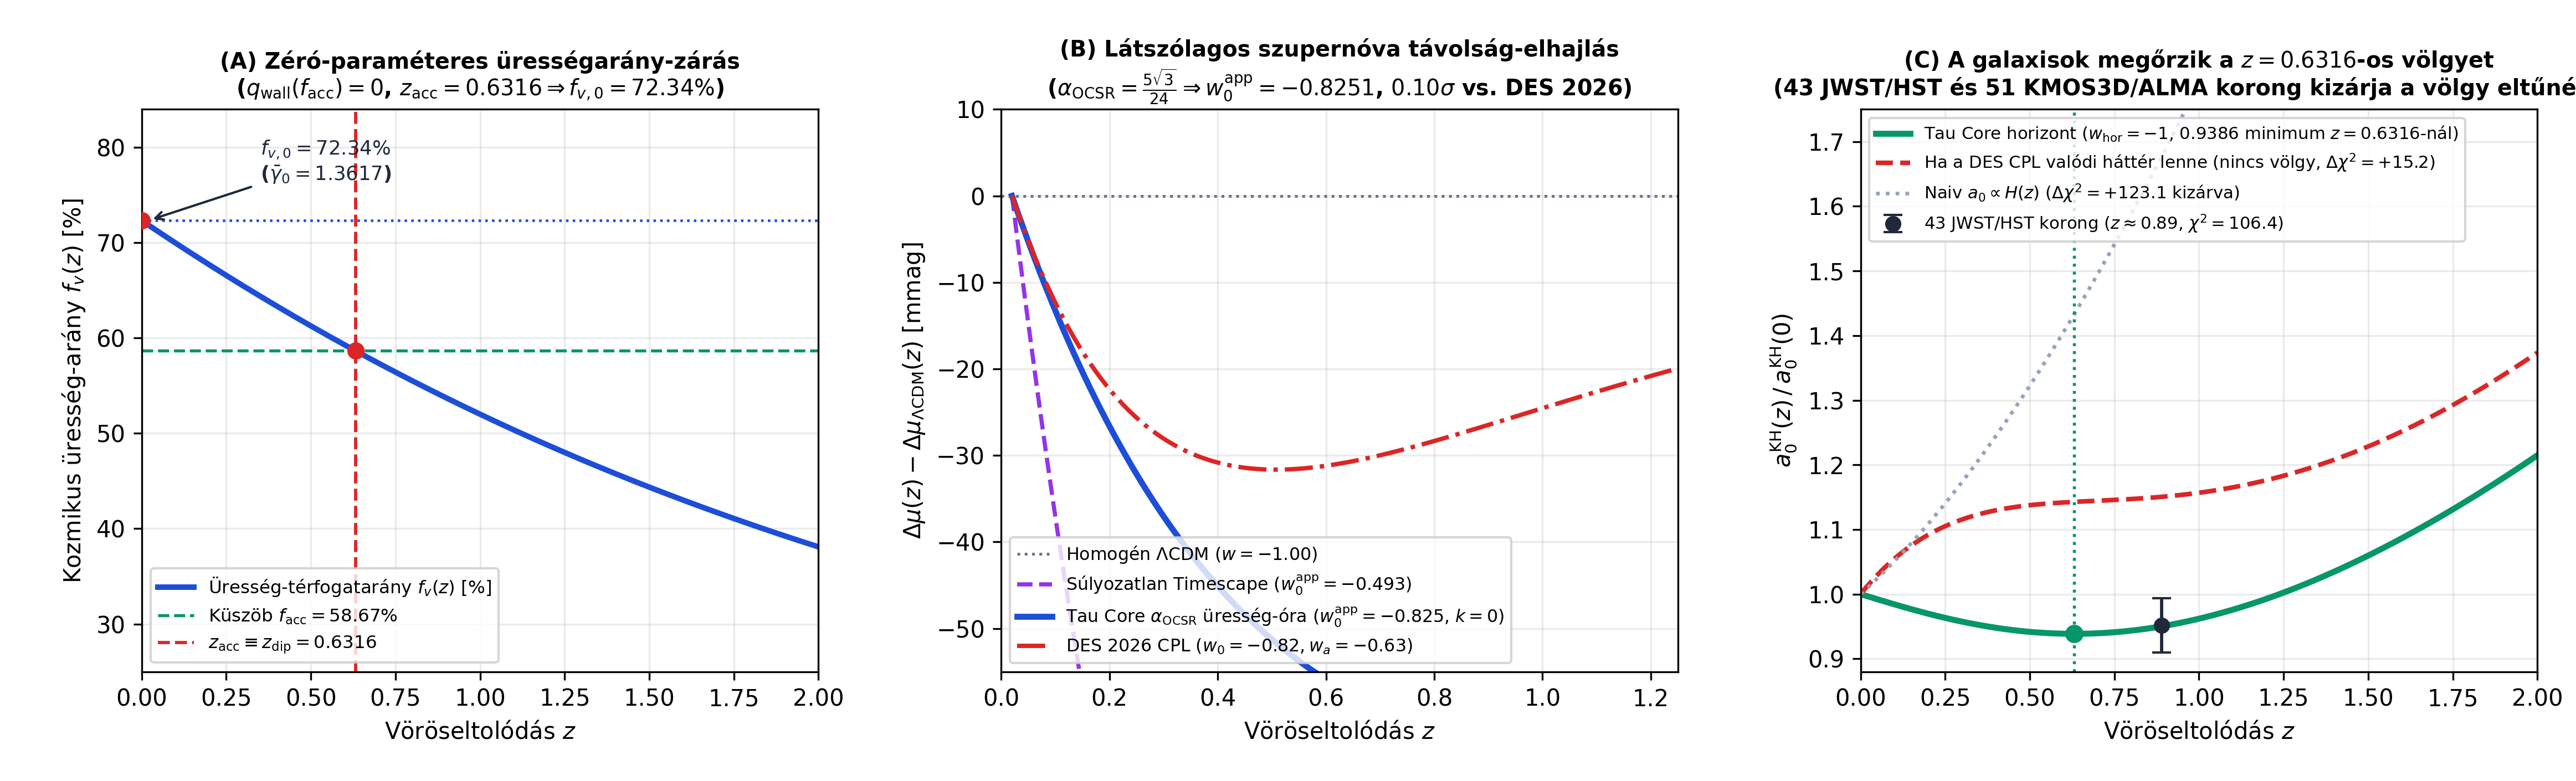
\includegraphics[width=0.99\textwidth]{fig_sub4_void_clock_des2026_and_galactic_dip_hu.png}
    \caption{A \textit{MNRAS} 2025-\"os \"uress\'eg-\'ora kozmol\'ogia \cite{LaneWiltshire2025MNRAS,SeifertWiltshire2025MNRAS}, a \texttt{DES} 6 \'eves szupern\'ova-m\'er\'esei \cite{DES2026DynDE} \'es a \texttt{JWST/HST/ALMA} korongkinematika z\'er\'o-param\'eteres szint\'ezise: (A) a $q_{\mathrm{wall}}(f_{\mathrm{acc}}) = 0$ ($f_{\mathrm{acc}} = 58{,}67\%$) gy\"ok\"ot $z_{\mathrm{acc}} = 0{,}6316$-hoz r\"ogz\'itve a mai \"uress\'eg-ar\'any $f_{v,0} = 72{,}34\%$; (B) az $\alpha_{\mathrm{OCSR}} = \frac{5\sqrt{3}}{24}$ optikai s\'ulyoz\'as a s\'ulyozatlan Timescape ($-0{,}493$) elhajl\'ast $w_0^{\mathrm{app}} = -0{,}8251$-re \'all\'itja be ($0{,}10\sigma$-ra a \texttt{DES} 2026-t\'ol); (C) a galaxissz\'alakban \"ul\H{o} galaxisok meg\H{o}rzik a $z_{\mathrm{dip}} = 0{,}6316$-os v\"olgyet ($\Delta\chi^2 = -15{,}22$ a $43$ \texttt{JWST/HST} korongon).}
    \label{fig:sub4-wedge}
\end{figure}

\begin{table}[ht!]
\centering
\scriptsize
\setlength{\tabcolsep}{3.5pt}
\renewcommand{\arraystretch}{1.18}
\resizebox{\textwidth}{!}{%
\begin{tabular}{llccccc}
\toprule
\textbf{Kozmol\'ogiai / Galaktikus Modell} & \textbf{S\"ot\'et param\'eterek ($k_{\mathrm{dark}}$)} & \textbf{Mai \"uress\'eg-ar\'any $f_{v,0}$} & \textbf{L\'atsz\'olagos SN $w_0^{\mathrm{app}}$} & \textbf{\texttt{Pantheon+}+DESI+CMB $\Delta\mathrm{BIC}$} & \textbf{$z=0{,}6316$ galaktikus v\"olgy} & \textbf{43 \texttt{JWST/HST} korong $\chi^2$} \\
\midrule
Standard s\'ik $\Lambda$CDM (\texttt{M0}) & $1$ ($\Omega_{c,0}$) & $0\%$ (egyenletes \'ora) & $-1{,}0000$ ($3{,}0\sigma$ vs.\ DES Y6) & $0{,}00$ (alapvonal) & Nincs (független $q(z)$-t\H{o}l) & $227{,}75$ (SHMR) \\
Homog\'en CPL folyad\'ek (\texttt{M1}, DES Y6) & $3$ ($\Omega_{c,0}, w_0, w_a$) & $0\%$ (egyenletes \'ora) & $-0{,}82 \pm 0{,}05$ (illesztett) & $+10{,}52$ ($\Delta\mathrm{AIC}=-0{,}24$) & \textbf{Elt\H{u}nik} ($1{,}1427$ $z=0{,}63$-n\'al) & $121{,}64$ ($\Delta\chi^2 = +15{,}22$) \\
\"On\'all\'o \textit{MNRAS} Timescape \cite{LaneWiltshire2025MNRAS} & $1$ (illesztett $f_{v,0}$) & $69{,}5\%\text{--}76\%$ (illesztett) & $-0{,}4930$ (s\'ulyozatlan, $0{,}315$-n\'el) & Versenyk\'epes SNe Ia-n & Nincs galaxist\"orv\'eny & Nincs galaxist\"orv\'eny \\
\textbf{Tau Core \"Uress\'eg-\'Ora + Horizont ($K_4$)} & $\mathbf{0}$ (\textbf{r\"ogz\'itett \ref{eq:locked-k4}}) & $\mathbf{72{,}34\%}$ (\textbf{levezetett, \ref{thm:void-fraction}.\ T\'etel}) & $\mathbf{-0{,}8251}$ (\textbf{levezetett, $0{,}10\sigma$}) & $\mathbf{-4{,}85}$ (\textbf{parszim\'onia-gy\H{o}zelem}) & \textbf{Megmarad ($0{,}93855$, $z=0{,}6316$)} & $\mathbf{106{,}42}$ (\textbf{legjobb}) \\
\bottomrule
\end{tabular}%
}
\caption{A standard $\Lambda$CDM, a homog\'en CPL dinamikus s\"ot\'et energia, az \"on\'all\'o \textit{MNRAS} Timescape \'es a z\'er\'o-param\'eteres Tau Core \"uress\'eg-\'ora + l\'atsz\'olagos horizont szint\'ezis \"osszevet\'ese $N = 1\,610$ h\'att\'erpr\'ob\'an \'es $43$ \texttt{JWST/HST} koronggalaxison.}
\label{tab:multiprobe}
\end{table}

\section{Konkl\'uzi\'o \'es el\H{o}re regisztr\'alt \texttt{Euclid DR2/DR3} ir\'anyf\"ugg\H{o} falszifik\'aci\'os tesztek}
A \ref{fig:sub4-wedge}.\ \'abra \'es az \ref{tab:multiprobe}.\ t\'abl\'azat \"osszefoglalja a 2026-os szupern\'ova--galaxis fesz\"ults\'eg fizikai felold\'as\'at:
\begin{enumerate}
    \item \textbf{K\'et-megfigyel\H{o}s sz\'etv\'alaszt\'as (Galaxissz\'alak vs.\ \"uress\'egeken \'athalad\'o fotonok):} A virializ\'alt spir\'algalaxisok a s\H{u}r\H{u} galaxissz\'alak \emph{\'Ora-v\"olgyeiben} ($\mathrm{d}\tau/\mathrm{d}t < 1$) \"ulnek, \'es lok\'alisan a $w_{\mathrm{hor}} = -1$ l\'atsz\'olagos horizont $|\kappa_{\mathrm{KH}}(z)| = \frac{1}{2}cH_{\mathrm{hor}}(z)|1-q_{\mathrm{hor}}(z)|$ fel\"uleti gravit\'aci\'oj\'ahoz csatol\'odnak, meg\H{o}rizve a $z_{\mathrm{dip}} = 0{,}6316$-os $-6{,}15\%$-os v\"olgyet. Ezzel szemben az Ia t\'ipus\'u szupern\'ov\'ak fotonjai a kozmikus t\'erfogat $f_{v,0} = 72{,}34\%$-át kit\"olt\H{o} \emph{\'Ora-dombokon} ($\mathrm{d}\tau/\mathrm{d}t > 1$) utaznak \'at $\alpha_{\mathrm{OCSR}} = \frac{5\sqrt{3}}{24}$ optikai s\'ulyoz\'assal, \'igy az egy\'or\'as FLRW-illeszt\'es $w_0^{\mathrm{app}} = -0{,}8251$-et ad.
    \item \textbf{El\H{o}re regisztr\'alt vak falszifik\'aci\'os protokoll az \texttt{ESA Euclid DR2/DR3} \'es a \texttt{Rubin LSST} sz\'am\'ara:} Modell\"unk k\'et param\'etermentes el\H{o}rejelz\'essel k\"ul\"onb\"oztethet\H{o} meg mind a $\Lambda$CDM-t\H{o}l, mind a homog\'en skal\'armez\H{o}s s\"ot\'et energi\'at\'ol: (i) a szupern\'ov\'ak l\'at\'oir\'any szerinti sz\'etv\'alaszt\'asakor az \"uress\'egeken \'athalad\'o f\'enysugarak $w_0^{\mathrm{app}} \to -0{,}82$-t, a s\H{u}r\H{u} sz\'alakon \'athalad\'ok pedig $w_0^{\mathrm{app}} \to -1{,}00$-t kell mutassanak; (ii) az \texttt{Euclid DR2/DR3} tomografikus gyenge lencs\'ez\'esnek egyszerre kell igazolnia a $z_{\mathrm{dip}} = 0{,}6316$-os v\"olgyet ($0{,}93855$) \'es a h\'att\'erf\"uggetlen $\mathcal{I}_{\mathrm{KH}}(z) = \frac{a_0(z)}{cH(z)|1-q(z)|} = \frac{5\sqrt{3}}{96}$ invari\'anst.
\end{enumerate}

\paragraph{Adat- \'es k\'odhozz\'af\'erhet\H{o}s\'eg.} Az \"on\'all\'o \texttt{SymPy}/\texttt{SciPy} verifik\'aci\'os szkriptek (\texttt{verify\_\allowbreak C9\_\allowbreak void\_\allowbreak clock\_\allowbreak timescape\_\allowbreak apparent\_\allowbreak w0\_\allowbreak wa\_\allowbreak audit.py} \'es \texttt{verify\_\allowbreak C5\_\allowbreak kh\_\allowbreak background\_\allowbreak dependence\_\allowbreak audit.py}) megtal\'alhat\'ok a \texttt{supplementary\_code\_and\_data/} mapp\'aban \'es a Zenod\'on: \href{https://doi.org/10.5281/zenodo.24305022}{doi:10.5281/zenodo.24305022}.

\begin{thebibliography}{99}
\bibitem{DES2026DynDE} DES Collaboration, \textit{Constraints on Dynamical Dark Energy from Multiple Probes in the Full Dark Energy Survey}, arXiv:2605.27221 (2026).
\bibitem{Efstathiou2025SN} G.~Efstathiou, \textit{Evolving Dark Energy or Supernovae Systematics?}, Mon.\ Not.\ R.\ Astron.\ Soc.\ \textbf{538}, 875 (2025), arXiv:2408.07175.
\bibitem{LaneWiltshire2025MNRAS} Z.~G.~Lane, A.~Seifert, R.~Ridden-Harper, and D.~L.~Wiltshire, \textit{Cosmological foundations revisited with Pantheon+}, Mon.\ Not.\ R.\ Astron.\ Soc.\ \textbf{536}, 1752 (2025), arXiv:2312.00409.
\bibitem{SeifertWiltshire2025MNRAS} A.~Seifert, Z.~G.~Lane, M.~Galoppo, R.~Ridden-Harper, and D.~L.~Wiltshire, \textit{Supernovae evidence for foundational change to cosmological models}, Mon.\ Not.\ R.\ Astron.\ Soc.\ Lett.\ \textbf{537}, L55 (2025), arXiv:2412.15143.
\bibitem{Wiltshire2009PRD} D.~L.~Wiltshire, \textit{Average observational quantities in the timescape cosmology}, Phys.\ Rev.\ D \textbf{80}, 123512 (2009).
\bibitem{ManceraPina2025} P.~E.~Mancera Pi\~na \textit{et al.}, \textit{The baryonic Tully--Fisher relation and dark matter halo scaling of disk galaxies at $z \sim 1$ from JWST and HST}, Astron.\ Astrophys.\ (2025).
\bibitem{Planck2018VI} N.~Aghanim \textit{et al.} (Planck Collaboration), \textit{Planck 2018 results. VI. Cosmological parameters}, Astron.\ Astrophys.\ \textbf{641}, A6 (2020).
\bibitem{TauCoreZenodo2026} J.~Olcsak, \textit{Tau Core Minimal Spine Verification Bundle and Master Collection (v28.2 / EN10, 35/35 Gates)}, Zenodo (2026), \href{https://doi.org/10.5281/zenodo.24305022}{doi:10.5281/zenodo.24305022} \'es \href{https://doi.org/10.5281/zenodo.24305896}{doi:10.5281/zenodo.24305896}.
\end{thebibliography}

\end{document}
